% replace all text with your own text.
% in this template few examples are mention
\chapter{Material and Methods}
\label{ch:method} % Label for method chapter



This chapter outlines the methodology used to analyse and compare the environmental impact of electric and petrol cars.
 Although electric vehicles (EVs) are often perceived as environmentally friendly,
 this study aims to demonstrate that they also contribute to pollution, but in different ways.
 The focus is on lifecycle emissions, including battery production, electricity generation, and fuel consumption.\\ 

To comprehensively analyse the environmental impacts of producing and operating electric vehicles, a Life Cycle Assessment (LCA)\href{https://www.sciencedirect.com/science/article/pii/S0048969722019520}{(Koroma et al., 2022)} approach is integrated into this study. LCA  helps evaluate the environmental footprint of both petrol and electric cars by considering all stages of their life cycle, from raw material extraction and manufacturing to usage and end-of-life disposal. This method provides a holistic view of the emissions and resource consumption associated with each vehicle type. By incorporating LCA, this study aims to assess not only direct emissions but also the hidden environmental costs linked to raw material extraction, battery production, and energy generation. \\
 
 A data analysis approach was adopted, using real-world datasets from
reputable sources such as the UK Government and the European Union \href{https://www.gov.uk/co2-and-vehicle-tax-tools}{(Government Digital Service, 2012)} . Previous studies have focused primarily on CO$_2$ emissions and air pollution caused by petrol cars, highlighting their impact on climate change.
 However, fewer studies have addressed the environmental costs of battery production and electric vehicle consumption. To provide a balanced comparison, this study examines
CO$_2$ emissions per mile, energy consumption, and impact on the life cycle of both vehicle types.
Data pre-processing and analysis are performed using Python, while visualization tools such
as Tableau or seaborn are used to present key findings and representing graphs showing the comparison and 
the similarities of this. 

The methodology of this study follows a structured, systematic process to ensure the accuracy, reliability, and comprehensiveness of data analysis and visualization. The approach is divided into distinct phases, each designed to build upon the previous step, facilitating a clear and logical progression toward answering the research question
\clearpage

\section{Data Collection}
 The first step of this study involves gathering relevant information and datasets that provides insights into vehicle emissions, battery production impact, and energy consumption. \\ To ensure data reliability, the sources are carefully selected from different well-known organizations. 
 \begin{itemize}
     \item \textbf{Vehicle emission and Energy Consumption} - This dataset \href{https://www.gov.uk/co2-and-vehicle-tax-tools}{(Government Digital Service, 2012)} includes comprehensive details on CO$_2$ emissions, NOx emissions, hydrocarbon emissions, and other pollutants for both petrol and electric vehicles. Additionally, it provides energy consumption figures, with electric vehicles measured in miles per kWh and Wh/km, while petrol cars include fuel efficiency under various driving conditions. This dataset helps in understanding the environmental footprint of different vehicle types by comparing energy efficiency, pollutant emissions, and range capabilities. Furthermore, it allows for a quantitative analysis of sustainability by examining lifecycle emissions and energy use trends.
 \end{itemize}

 \begin{figure}[H]
    \centering
    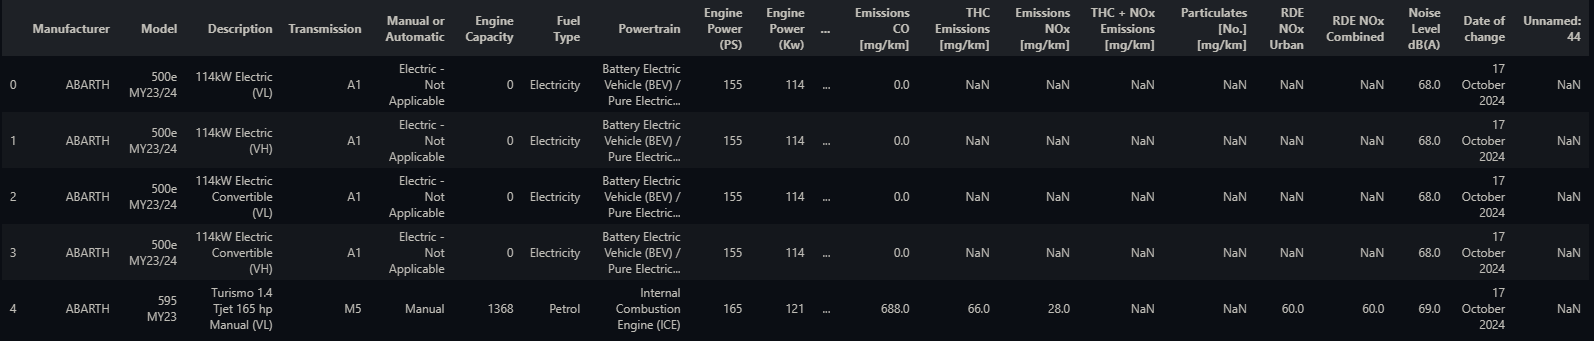
\includegraphics[scale=0.38]{figures/Vehicle Emissions.png}
    \caption{\textit{Snapshot Clean data new table \LaTeX}.}
    \label{fig:chart_1}
\end{figure}
\begin{itemize}
    \item \textbf{Battery Production} - 
\end{itemize}
 


\section{Data Processing}
\begin{lstlisting}[language=Python, caption={Code snippet in \LaTeX ~and  this is a Python code }, label=list:python_code_ex]
import pandas as pd

df = pd.read_csv("latestEuro6.csv", encoding="ISO-8859-1")


#show all columns
print(df.columns)
\end{lstlisting}
\begin{figure}[H]
    \centering
    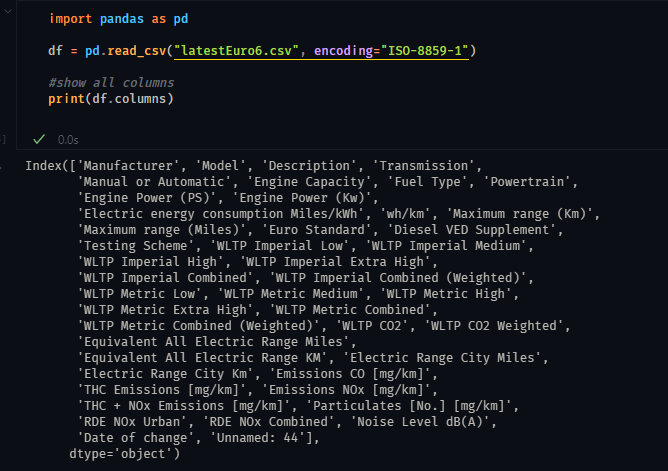
\includegraphics[scale=0.85]{figures/ColumnNames.png}
    \caption{\textit{Snapshot Column Names \LaTeX}.}
    \label{fig:chart_1}
\end{figure}

Firstly, the dataset it is not clean from unnecessary data, Figure ~\ref{list:python_code_list}. This shows the list of all the columns that the dataset have.

\begin{lstlisting}[language=Python, caption={Code snippet in \LaTeX ~and  this is a Python code, removind unnesesary data }, label=list:python_code_list]
import pandas as pd

df = pd.read_csv("latestEuro6.csv", encoding="ISO-8859-1")

# Remove unnecessary columns
df.drop(columns=["Unnamed: 44", "Date of change", "Description"], inplace=True)

# Fill missing electric range values with the median
df["Maximum range (Km)"].fillna(df["Maximum range (Km)"].median(), inplace=True)
df["Electric energy consumption Miles/kWh"].fillna(df["Electric energy consumption Miles/kWh"].median(), inplace=True)

df.drop_duplicates(inplace=True)

# Save the cleaned data to a new CSV file
df.to_csv("cleaned_dataset6.csv", index=False)

\end{lstlisting}

On this Figure \ref{list:python_code_list}, it shows the step by step that it took to clean and optimize the dataset, while keeping the important data, that will be use to demonstrate the theory. By removing empty and duplicates, removing unnecessary columns data, and adding on the missing values the median, will give us an approximation of how much are electric cars compare to Petrol car when comparing about environmental impact.


After all the cleaning process and the optimization of the dataset, it will look like this:
\begin{figure}[H]
    \centering
    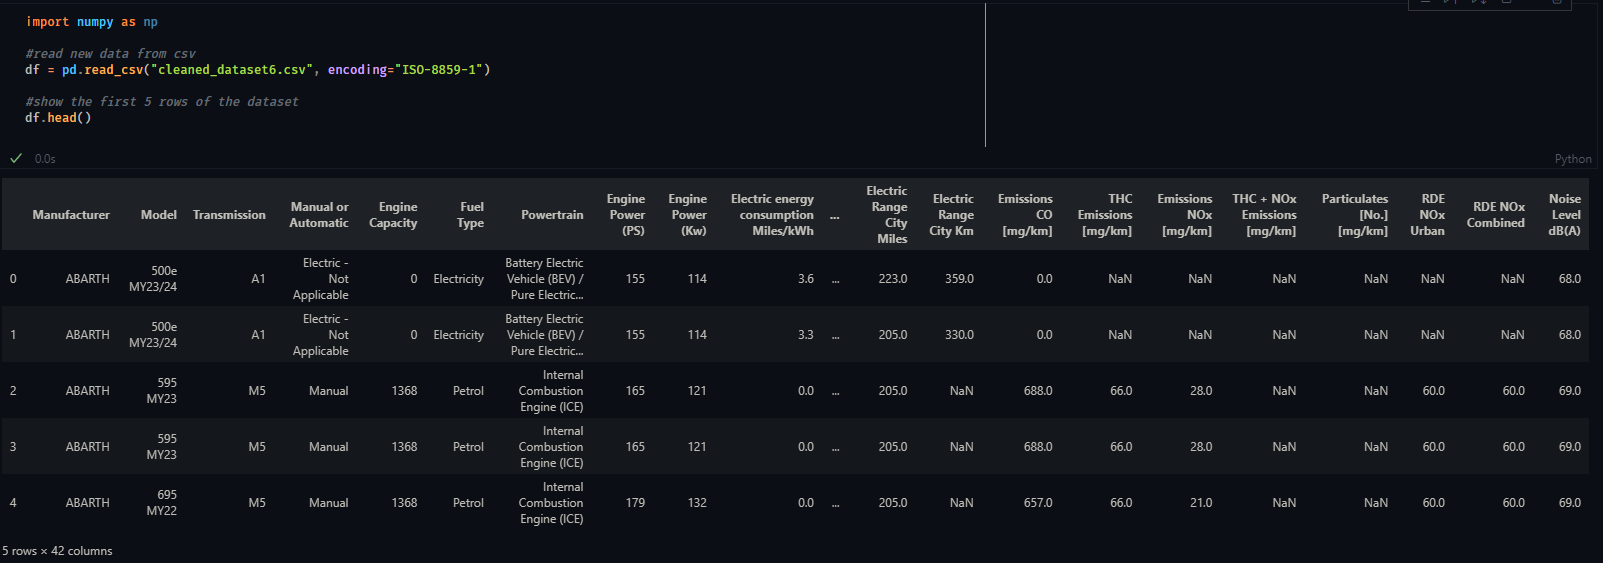
\includegraphics[scale=0.35]{figures/CleanData.png}
    \caption{\textit{Snapshot Clean data new table \LaTeX}.}
    \label{fig:chart_2}
\end{figure}

Having the dataset almost ready for the data analysis of the data.
            

\section{Example of a Figure in \LaTeX}
Figure~\ref{fig:chart_a} is an example of a figure in \LaTeX. For more details, check the link:

\href{https://en.wikibooks.org/wiki/LaTeX/Floats,_Figures_and_Captions}{wikibooks.org/wiki/LaTeX/Floats,\_Figures\_and\_Captions}.

\noindent
Keep your artwork (graphics, figures, illustrations) clean and readable. At least 300dpi is a good resolution of a PNG format artwork. However, an SVG format artwork saved as a PDF will produce the best quality graphics. There are numerous tools out there that can produce vector graphics and let you save that as an SVG file and/or as a PDF file. One example of such a tool is the ``Flow algorithm software''. Here is the link for that: \href{http://www.flowgorithm.org/download/}{flowgorithm.org}.
\begin{figure}[ht]
    \centering
    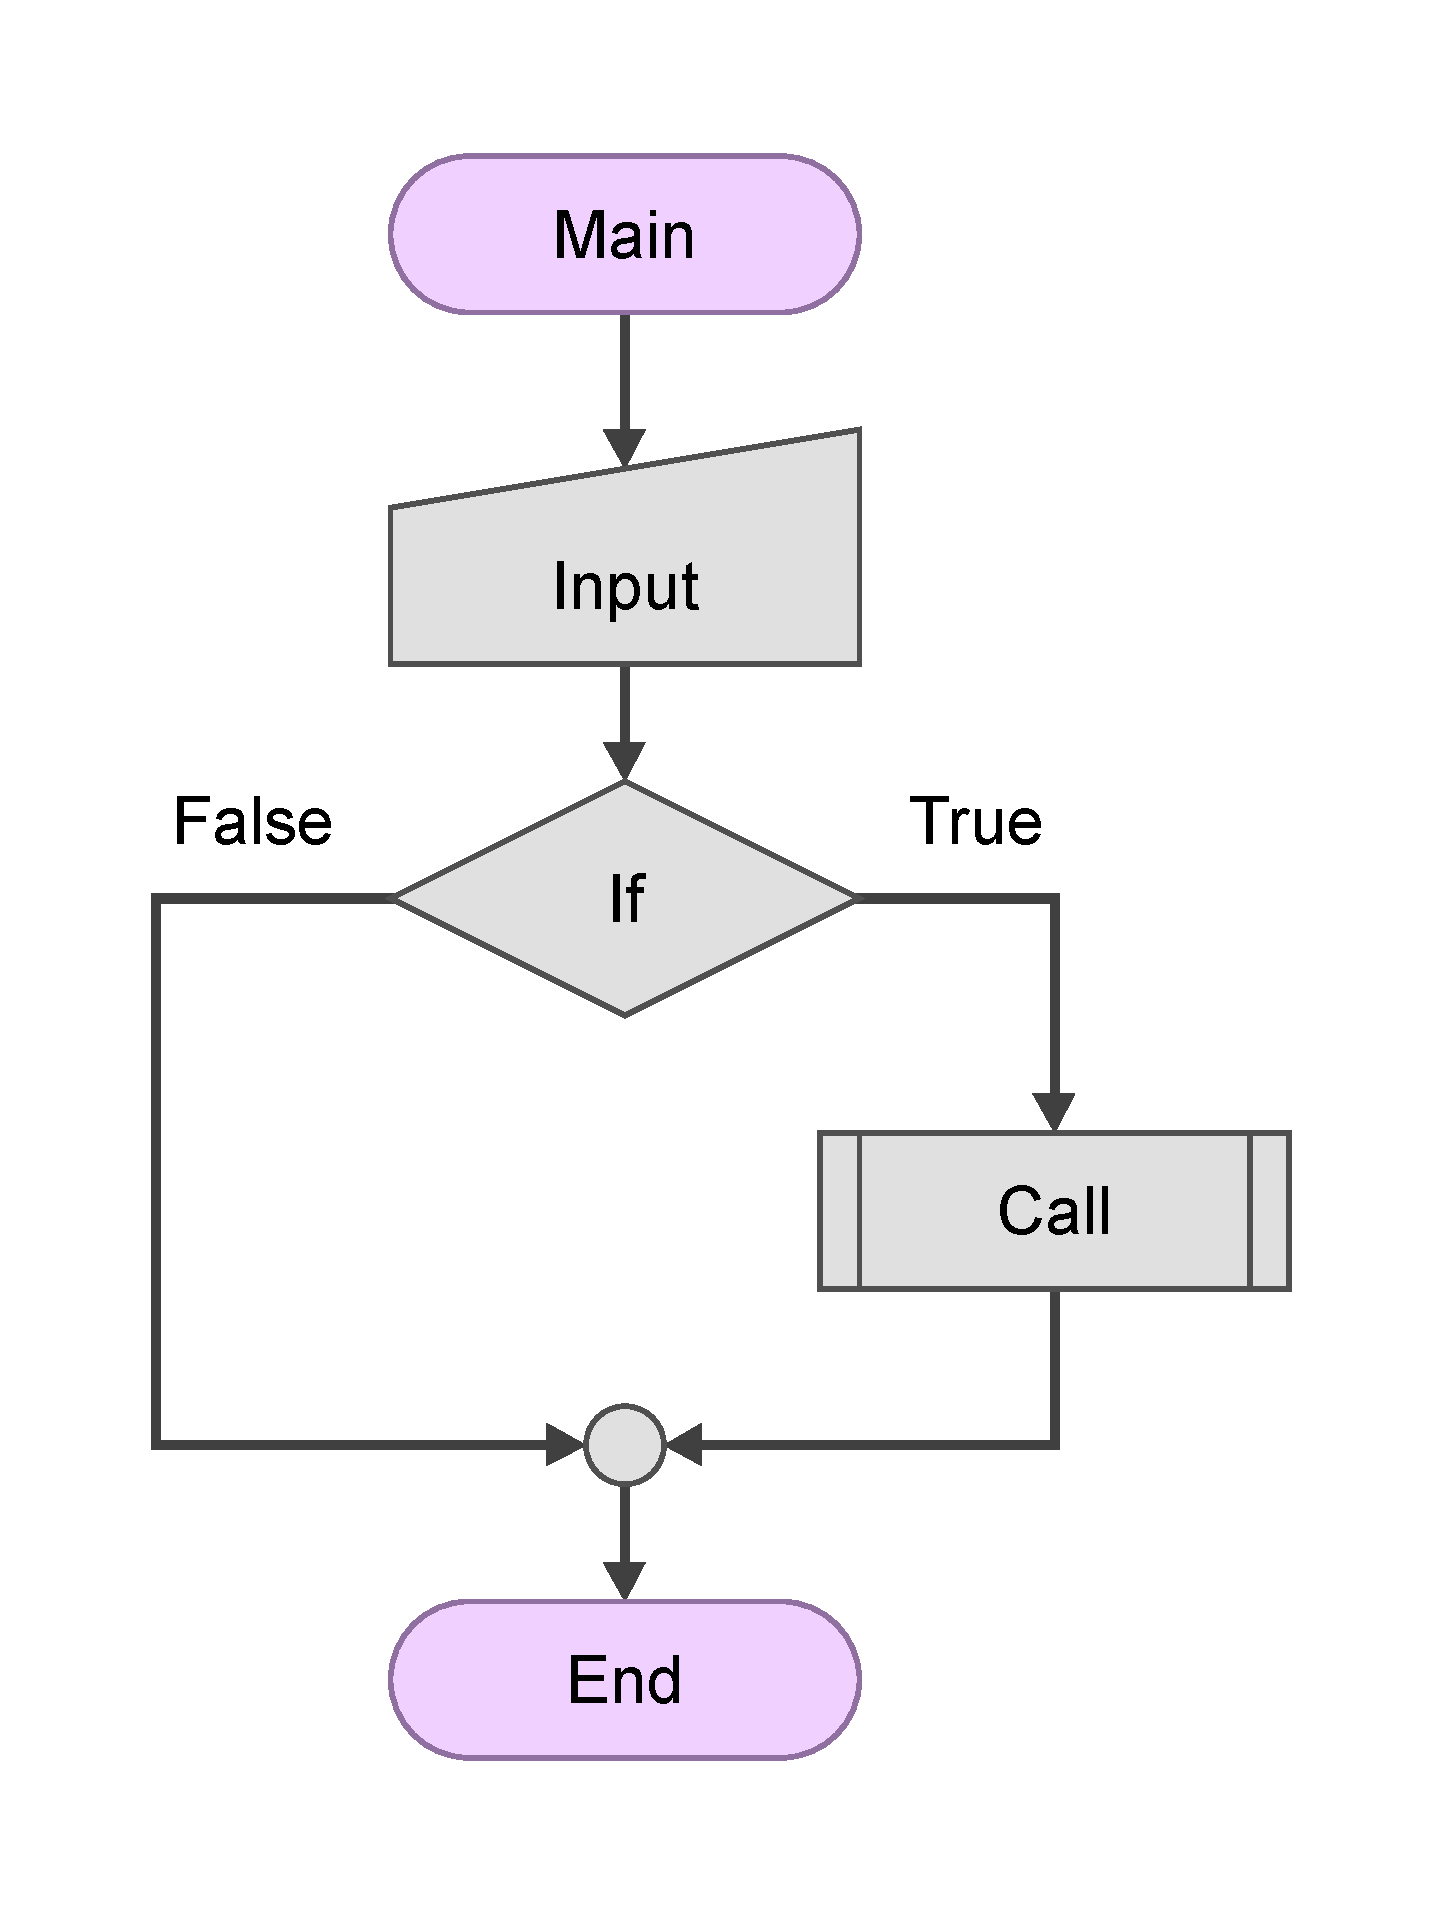
\includegraphics[scale=0.3]{figures/chart.pdf}
    \caption{Example figure in \LaTeX.}
    \label{fig:chart_a}
\end{figure}

\clearpage %  use command \clearpage when you want section or text to appear in the next page.

\section{Example of an algorithm in \LaTeX}
Algorithm~\ref{algo:algo_example} is a good example of an algorithm in \LaTeX.  
\begin{algorithm}
    \caption{Example caption: sum of all even numbers}
    \label{algo:algo_example}
    \begin{algorithmic}[1]
        \Require{$ \mathbf{x}  = x_1, x_2, \ldots, x_N$}
        \Ensure{$EvenSum$ (Sum of even numbers in $ \mathbf{x} $)}
        \Statex
        \Function{EvenSummation}{$\mathbf{x}$}
        \State {$EvenSum$ $\gets$ {$0$}}
        \State {$N$ $\gets$ {$length(\mathbf{x})$}}
        \For{$i \gets 1$ to $N$}                    
        \If{$ x_i\mod 2 == 0$}  \Comment check if a number is even?
        \State {$EvenSum$ $\gets$ {$EvenSum + x_i$}}
        \EndIf
        \EndFor
        \State \Return {$EvenSum$}
        \EndFunction
    \end{algorithmic}
\end{algorithm}
 
\section{Example of code snippet  in \LaTeX}

Code Listing~\ref{list:python_code_ex} is a good example of including a code snippet in a report. While using code snippets, take care of the following:
\begin{itemize}
    \item do not paste your entire code (implementation) or everything you have coded. Add code snippets only. 
    \item The algorithm shown in Algorithm~\ref{algo:algo_example} is usually preferred over code snippets in a technical/scientific report. 
    \item Make sure the entire code snippet or algorithm stays on a single page and does not overflow to another page(s).  
\end{itemize}

Here are three examples of code snippets for three different languages (Python, Java, and CPP) illustrated in Listings~\ref{list:python_code_ex}, \ref{list:java_code_ex}, and \ref{list:cpp_code_ex} respectively.  

\begin{lstlisting}[language=Python, caption={Code snippet in \LaTeX ~and  this is a Python code example}, label=list:python_code_ex]
import numpy as np

x  = [0, 1, 2, 3, 4, 5] # assign values to an array
evenSum = evenSummation(x) # call a function

def evenSummation(x):
    evenSum = 0
    n = len(x)
    for i in range(n):
        if np.mod(x[i],2) == 0: # check if a number is even?
            evenSum = evenSum + x[i]
    return evenSum
\end{lstlisting}

Here we used  the ``\textbackslash clearpage'' command and forced-out the second listing example onto the next page. 
\clearpage  %
\begin{lstlisting}[language=Java, caption={Code snippet in \LaTeX ~and  this is a Java code example}, label=list:java_code_ex]
public class EvenSum{ 
    public static int evenSummation(int[] x){
        int evenSum = 0;
        int n = x.length;
        for(int i = 0; i < n; i++){
            if(x[i]%2 == 0){ // check if a number is even?
                evenSum = evenSum + x[i];
            }
        }
        return evenSum;     
    }
    public static void main(String[] args){ 
        int[] x  = {0, 1, 2, 3, 4, 5}; // assign values to an array
        int evenSum = evenSummation(x);
        System.out.println(evenSum);
    } 
} 
\end{lstlisting}


\begin{lstlisting}[language=C, caption={Code snippet in \LaTeX ~and  this is a C/C++ code example}, label=list:cpp_code_ex]
int evenSummation(int x[]){
    int evenSum = 0;
    int n = sizeof(x);
    for(int i = 0; i < n; i++){
        if(x[i]%2 == 0){ // check if a number is even?
            evenSum = evenSum + x[i];
    	}
    }
    return evenSum;     
}

int main(){
    int x[]  = {0, 1, 2, 3, 4, 5}; // assign values to an array
    int evenSum = evenSummation(x);
    cout<<evenSum;
    return 0;
}
\end{lstlisting}



\section{Example of in-text citation style}
\subsection{Example of the equations and illustrations placement and reference in the text}
Make sure whenever you refer to the equations, tables, figures, algorithms,  and listings for the first time, they also appear (placed) somewhere on the same page or in the following page(s). Always make sure to refer to the equations, tables and figures used in the report. Do not leave them without an \textbf{in-text citation}. You can refer to equations, tables and figures more them once.

\subsection{Example of the equations and illustrations style}
Write \textbf{Eq.} with an uppercase ``Eq`` for an equation before using an equation number with (\textbackslash eqref\{.\}). Use ``Table'' to refer to a table, ``Figure'' to refer to a figure, ``Algorithm'' to refer to an algorithm and ``Listing'' to refer to listings (code snippets). Note that, we do not use the articles ``a,'' ``an,'' and ``the'' before the words Eq., Figure, Table, and Listing, but you may use an article for referring the words figure, table, etc. in general.

For example, the sentence ``A report structure is shown in \textbf{the} Table~\ref{tab:gen_template}'' should be written as ``A report structure is shown \textbf{in} Table~\ref{tab:gen_template}.'' 
 

\section{Summary}
Write a summary of this chapter.

~\\[5em]
\noindent
{\huge\textbf{Note:}} In the case of \textbf{software engineering} project a Chapter ``\textbf{Testing and Validation}'' should precede the ``Results'' chapter. See Section~\ref{subsec:se_chpters} for report organization of such project. 

